\chapter{Przegląd literatury}
\section{Przegląd - notatki}

\subsection*{Mapping the global structure of TSP fitness landscapes (2018) \cite{DBLP:journals/heuristics/OchoaV18}}
Celem pracy było zbadanie przestrzeni rozwiązań różnych instancji problemu komiwojażera(TSP), oraz opracowanie
procedury próbkowania tych przestrzeni.
W pracy przedstawiony został algorytm próbkujący oparty o algorytm \textit{Chained-Lin-Kerninghan}.
Do próbkowania wykorzystano implementację tego algorytmu z biblioteki \textit{Concorde}.
Algorytm konstruuje sieć optimów lokalnych(LON) - odmianę z definicją krawędzi \textit{escape edges}.

Wykonane zostało 1000 niezależnych przebiegów algorytmu.
Połowa z nich korzystała z metody inicjalizacji Quicka-Borůvki, a druga połowa za punkt startowy przyjmowała losowe rozwiązanie.
Algorytm opiera się na generowaniu nowych rozwiązań poprzez zastosowanie perturbacji typu double-bridge,
a następnie uruchomieniu algorytmu Lin-Kerninghan, by znaleźć lokalne minimum.
Operacja jest powtarzana 10000 razy i budowana jest w ten sposób sieć optimów lokalnych.

Jednym z zadań, które postawili sobie autorzy pracy, była identyfikacja struktur lejowych w przestrzeni rozwiązań.
Lej jest sekwencją lokalnych optimów, których wartość dopasowania się nie pogarsza,
i która zmierza do pewnego optimum - globalnego (lej pierwszorzędny - ang. primary funnel) lub lokalnego (lej drugorzędny - ang. secondary funnel).
To optimum nazywane jest spodem leja (ang. funnel floor/bottom).

Sieci optimów lokalnych wygenerowane przez kolejne uruchomienia algorytmu próbkującego zawyżały liczbę lejów w przestrzeni rozwiązań.
Badacze scalili więc znalezione optima lokalne z wszystkich przebiegów algorytmu.
Znalezione w ten sposób rozwiązania nazwali atraktorami i utworzyli graf sieci atraktorów, w której są one wierzchołkami.
Następnie spody lejów zostały zidentyfikowane jako wierzchołki, z których nie ma krawędzi wychodzących.
Przynależność optimów lokalnych do poszczególnych lejów odbywała się poprzez sprawdzenie,
czy istnieje ścieżka w grafie pomiędzy danym optimum a spodem leja.

Do badań wykorzystano 20 instancji TSP o rozmiarach od 500 do 1500 miast.
Wykorzystano instancje o miastach rozłożonych równomiernie i w klastrach.
Część została wygenerowana losowo, a część pochodziła z biblioteki TSPLIB.

Zbadano właściwości powstałych sieci optimów lokalnych, m.in. liczbę unikalnych optimów lokalnych i globalnych, liczba wywołań funkcji celu,
stosunek liczby wierzchołków i wywołań funkcji celu, stosunek wierzchołków jest połączonych ścieżką
z optimum globalnym do całkowitej liczby wierzchołków, średnią siłę(ang. strength) wierzchołków.
Zbadano również własności lejów, takie jak rozmiar największego leja czy liczba atraktorów.

Badania wykazały, że przestrzeń rozwiązań badanych instancji TSP zawiera wiele lejów a nie, jak wcześniej sądzono,
jeden lej kończący się w globalnym minimum. W przestrzeni rozwiązań instancji o regularnej strukturze
wykryto istnienie rozległych płaskowyżów(ang. plateaus). Zauważono różnicę między instancjami wygenerowanymi losowo a rzeczywistymi.
Te pierwsze miały zwykle jedno globalne optimum i małą neutralność, podczas gdy instancje rzeczywiste
zwykle miały więcej globalnych optimów, czasem formujących płaskowyż globalnych optimów.
Zauważono zależność między rozmiarem instancji a liczbą lejów - ich liczba zwiększa się wraz ze wzrostem
rozmiaru instancji. Najwięcej lejów pojawiło się w instancjach z równomiernym losowym rozmieszczeniem miast.
Zbadano korelację między różnymi właściwościami przestrzeni rozwiązań.
Wykazano, że w instancjach, w których miasta rozmieszczone są w klastrach, występuje większa korelacja
właściwości, niż w instancjach o rozłożeniu równomiernym.

\subsection*{Local Optima Networks in Solving Algorithm Selection Problem for TSP (2018) \cite{DBLP:conf/depcos/BozejkoGNAB18}}
W pracy badano możliwość wykorzystania analizy sieci optimów lokalnych w problemie wyboru algorytmu heurystycznego dla danej instancji problemu komiwojażera
(Algorithm selection problem).

Wykorzystano algorytm dwufazowy (ang. Two-Phase Sampling).
Algorytm tego typu podzielony jest na dwa etapy - poszukiwanie wierzchołków i poszukiwanie krawędzi.
Wierzchołki wyszukiwane są poprzez generowanie losowych rozwiązań i uruchamianiu na nich algorytmu 2-opt typu best-improvement.
Algorytm generuje LON opartą o escape edges.
Próbkowanie krawędzi polega na poddaniu każdego ze znalezionych wcześniej lokalnych optimów perturbacji typu 2-change i
optymalizacji algorytmem 2-opt typu first-improvement.
Sprawdzany jest następnie warunek istnienia krawędzi i, jeśli jest spełniony, do zbioru dodawana jest odpowiednia krawędź
bądź zwiększana jest jej waga, jeśli już istnieje ona w zbiorze.
Wśród badanych parametrów wymienić można m.in stosunek liczby krawędzi do liczby wierzchołków,
średnia odległość optimum lokalnego od optimum o najniższej wartości funkcji celu,
stosunek wierzchołków połączonych z tym optimum do pozostałych oraz różnorodność(ang. assortativity) i współczynnik klasteryzacji grafu.
Do eksperymentów wykorzystano instancje problemu z biblioteki TSPLIB, oraz instancje generowane losowo o równomiernym rozkładzie miast.
Obliczono korelację różnych miar, aby wyeliminować redundantne dane.

Na każdej instancji problemu uruchomiono algorytmy heurystyczne i porównano parami jakość ich rozwiązań.
Obliczono również średnią względnej jakości rozwiązań dla każdego algorytmu.
Porównane zostały algorytmy \textit{Greedy Descent}, \textit{Guided Local Search}, \textit{Simulated Annealing}, \textit{Taboo Search}, \textit{Objective Taboo Search}.
Wykorzystano implementacje zawarte w pakiecie \textit{Google Optimization Tools}. Sprawdzono również obecny w pakiecie tryb automatyczny, który sam dobiera
algorytm dla danej instancji.

Na podstawie zebranych danych nauczono klasyfikatory dla każdej pary algorytmów.
Klasyfikatory przypisywały wyniki do jednej z trzech klas: 1 - algorytm A daje lepszy wynik od algorytmu B,
2 - algorytm B daje lepszy wynik od algorytmu A, 3 - algorytmy dają ten sam wynik.
Utworzone klasyfikatory porównano z klasyfikatorem ZeroR.
Przygotowane klasyfikatory dokonały poprawnej predykcji częściej niż ZeroR w przypadku instancji ze
zbioru TSPLIb. W przypadku instancji generowanych losowo, tylko w jednym przypadku klasyfikator
okazał się lepszy od ZeroR.

Eksperymenty wykazały, że analiza sieci optimów lokalnych może zostać z powodzeniem wykorzystana do
selekcji algorytmu heurystycznego, jednak czas próbkowania, dłuższy od czasu samego rozwiązywania problemu,
ogranicza jej użyteczność.

\subsection*{Clarifying the Difference in Local Optima Network Sampling Algorithms (2019) \cite{DBLP:conf/evoW/ThomsonOV19}}
W pracy wykonane zostało statystyczne porównanie dwóch algorytmów próbkowania
sieci lokalnych optimów dla kwadratowego problemu przydziału(QAP).
Do badań wykorzystano instancje problemu z biblioteki QAPLIB.
Wybrano 30 instancji o różnych klasach (rozłożone równomiernie, na siatce,
instancje rzeczywiste, instancje losowe symulujące rzeczywiste).
Porównano algorytmy \textit{Snowball} oraz \textit{Iterated Local Search}.
Spróbkowane dane wykorzystano do stworzenia modelów regresji do przewidywania jakości rozwiązań
dwóch algorytmów heurystycznych: \textit{Robust Taboo Search} Taillarda oraz \textit{Improved ILS} Stützla.

Wykonano próbkowanie przestrzeni rozwiązań i sprawdzono, czy wartości poszczególnych miar pochodzące od dwóch algorytmów
są ze sobą skorelowane.
Zbadanymi miarami były m.in: liczba optimów, liczba krawędzi, średnia liczba krawędzi wychodzących z wierzchołka grafu(ang. outdegree),
średnica grafu, średnie dopasowanie lokalnych optimów(ang. meanfitness), sinkfitness (dopasowanie spływów? TODO: translate).
Zauważono korelację metryk meanfitness i sinkfitness  na poziomie 0.99.
Dla wszystkich innych metryk korelacja było mniejsza od 0.5, dla średnicy grafu była ona ujemna.
Na podstawie zebranych danych nauczono modele typu liniowego oraz \textit{RandomForest}.
Zbadano wartości metryki $R^{2}$ dla różnych parametrów algorytmów próbkowania, algorytmów heurystycznych
i modelów regresji.
Obliczono również współczynniki korelacji pomiędzy różnymi właściwościami sieci lokalnych optimów
a performance gap metric(TODO: translate) algorytmów optymalizujących.

Badania wykazały, że sieci wygenerowane przez dwa różne algorytmy próbkujące mają pewne wspólne cechy.
\textit{Snowball} okazał się bardziej przewidywalny i łatwiejszy w dobieraniu parametrów.
ITS natomiast lepiej znajdował struktury skupiające (ang. hub-and-spoke structures, hubs) w przestrzeni rozwiązań.
Wartości metryk LON uzyskane na podstawie algorytmu ITS były bardziej skorelowane z
jakością rozwiązania heurystyki(ang. heuristic performance metric).
Modele regresji utworzone na podstawie danych uzyskanych z ITS dokonywały lepszej predykcji
jakości rozwiązań algorytmów heurystycznych, niż modele utworzone na podstawie algorytmu Snowball.
Zauważono, że wartości funkcji celu w poszczególnych lokalnych optimach sieci LON
były lepszymi predyktorami, niż informacje o krawędziach tej sieci.

\subsection*{Inferring Future Landscapes: Sampling the Local Optima Level (2020) \cite{DBLP:journals/ec/ThomsonOVV20}}
W pracy zostały porównane algorytmy próbkowania sieci optimów lokalnych(LON) dla kwadratowego problemu przydziału (QAP).
Porównane zostały algorytmy \textit{Markov-Chain} oraz \textit{Snowball}.
Dla małych instancji problemu wykonano kompletne przeszukanie przestrzeni rozwiązań,
dla większych - przeszukiwanie z limitowanym budżetem obliczeniowym.

Jako instancje testowe wykorzystano przykłady ze zbioru QAPLIB.
Instancje należały do pięciu kategorii: instancje z wartościami losowymi z rozkładu równomiernego,
instancje z wartościami odległości ułożonymi "na siatce" i losowymi wartościami przepływu, rzeczywiste instancje problemu,
instancje generowane symulujące rzeczywiste, oraz instancje nie pasujące do żadnej z poprzednich kategorii.

Badane właściwości sieci LON różniły się w zależności od algorytmu próbkowania.
Dla Algorytmu \textit{Markov-chain} były to: liczba wierzchołków i krawędzi grafu, średnie dopasowanie(ang. meanfitness),
średnia liczba krawędzi wychodzących z wierzchołka (ang. mean outdegree), oraz najdłuższa ścieżka między wierzchołkami.
Dodatkowo zbadano tzw. metryki lejowe(ang. Funnel metrics) - liczba krawędzi do globalnego optimum (ang. incoming global)
oraz średnie dopasowanie spodu leja(ang. mean funnel-floor fitness).

Dla algorytmu \textit{Snowball} metryki lejowe, oraz te oparte o gęstość i wzory połączeń krawędzi nie dają użytecznych informacji,
zamiast tych metryk wybrano: średnią wagę pętli w grafie, średnią różnicę wag krawędzi wychodzących (ang. mean weight disparity),
korelację dopasowania między sąsiadami (ang. fitness-fitness correlation), średnia długość "wspinaczki" do optimum lokalnego,
maksymalna długość "wspinaczki" do lokalnego optimum oraz maksymalna liczba ścieżek prowadzących do lokalnego optimum.

Na podstawie danych zbudowano modele regresji, dokonujące predykcji jakości rozwiązań
uzyskanych przy wykorzystaniu heurystyk \textit{Improved Iterated Local Search} i \textit{Robust Taboo Search}.
Sprawdzono modele liniowe i \textit{RandomForest}. Modele oparte o \textit{RandomForest} okazały się lepsze.

Badania nie wykazały wyższości jednego algorytmu próbkowania nad drugim. Autorzy zwracają uwagę na fakt, że niektóre z cech
sieci optimów lokalnych są lepiej odwzorowywane przez algorytm \textit{Markov-chain}, a inne lepiej przez \textit{Snowball}.
Najlepsze wśród zbudowanych modeli regresji okazały się zaś te, które korzystały z kombinacji danych pozyskanych z obu algorytmów.

\subsection*{Understanding AutoML Search Spaces with Local Optima Networks (2022) \cite{DBLP:conf/gecco/TeixeiraP22}}
AutoML jest procesem automatyzacji konfiguracji procesów(pipelines) uczenia maszynowego.
Może obejmować on takie zadania jak wstępne przetwarzanie danych, ekstrakcja cech, dobór odpowiedniego algorytmu i jego hiperparametrów.
Mnogość możliwych konfiguracji procesu sprawia, że przestrzeń przeszukiwania AutoML jest duża.
W opisanej pracy autorzy podejmują próbę analizy przestrzeni AutoML dla zadania klasyfikacji przy wykorzystaniu sieci optimów lokalnych.

Przestrzeń przeszukiwania AutoML cechuje się dużą liczbą parametrów warunkowych - parametrów, których istnienie zależy od wartości innych parametrów.
Jest to spowodowane tym, że algorytmy uczenia maszynowego przyjmują inny zestaw hiperparametrów.
Z tego powodu do reprezentacji przestrzeni rozwiązań wykorzystano odpowiednią gramatykę BNF z rozwiązaniami generowanymi
przy użyciu drzewa wyprowadzania gramatyki (grammar derivation tree).
Powstała gramatyka posiada 38 reguł decydujących o zastosowanych algorytmach wstępnego przetwarzania danych,
zastosowanego algorytmu klasyfikacji oraz jego hiperparametrów.
Spośród algorytmów klasyfikacji wykorzystano: Regresję logistyczną, MLP, KNN, Random Forest i Ada Boost.

Wierzchołki LON zdefiniowano jako lokalne maksima przestrzeni rozwiązań.
Jako wartość dopasowania wybrano uśrednioną wartość metryki F-score dla danej konfiguracji procesu.
Sąsiedztwo rozwiązania zdefiniowano jako zbiór rozwiązań możliwych do uzyskanie poprzez zastosowanie operatora
mutacji na danym rozwiązaniu. Za operator mutacji przyjęto losowe wybranie jednego wierzchołka z drzewa rozwiązania
i zastąpienie go losowym drzewem (przy zachowaniu zasad gramatyki procesu). Szansa na wylosowanie wierzchołka
została uzależniona od głębokości jego pozycji w drzewie. W ten sposób operacje zmieniające proces w znaczny sposób
(np. zmiana algorytmu) mają mniejsze prawdopodobieństwo wystąpienia niż operacje zmieniające jedynie wartość hiperparametrów.
Zbudowano sieci oparte o 3 różne definicje krawędzi - basin-transition edges, escape edges i perturbation edges.
Do próbkowania przestrzeni rozwiązań w celu utworzenia LON wykorzystano algorytm wstępujący(hill-climb).

Do badań wykorzystano 7 zbiorów danych, zbadano 30 różnych przestrzeni konfiguracji.
Ze względu na złożoność obliczeniową badania sąsiedztwa, próbkowano ograniczoną liczbę sąsiadów.
Parametr ten nazwano wielkością sąsiedztwa i zbadano 4 warianty - 20, 30, 50 i 100 sąsiadów.
W każdym przypadku wartość dopasowania została obliczona dla wszystkich rozwiązań w przestrzeni.
Nadano budżet 120 sekund na wykonanie obliczeń określających wartość dopasowania danego rozwiązania.
W przypadku przekroczenia otrzymywał on wartość 0.

Zbadano korelację między wartością dopasowania optimum lokalnego a rozmiarem jego basenu przyciągania w zależności
od rozmiaru sąsiedztwa. Wykazano, że istnieje silna korelacja i zwiększanie sąsiedztwa w większości przypadków zmniejsza liczbę
basenów przyciągania w przestrzeni i zwiększa rozmiar istniejących.
Ta zależność nie zachodziła jednak w przypadku jednego z badanych zbiorów danych.

Zauważono wpływ zastosowanej definicji krawędzi na powstałą sieć LON - w sieciach z krawędziami typu
basin-transition nie zauważono obecności ścieków (wierzchołków bez krawędzi wychodzących, ang. sinks),
natomiast istniało wiele źródeł (wierzchołków bez krawędzi wchodzących, ang. sources).
Ilość źródeł zmniejszała się wraz ze wzrostem sąsiedztwa.
Sieci oparte o escape edges miały natomiast dużo ścieków i mało źródeł.
Zwiększanie rozmiaru sąsiedztwa prowadziło do zmniejszenia liczby ścieków.
Podobny efekt dawało zwiększenie parametru D.
W przypadku perturbation edges w sieci nie było ścieków ani źródeł niezależnie od rozmiaru sąsiedztwa.

Obliczono odległości między parami lokalnych i globalnych optimów.
Stwierdzono, że odległości między optimami globalnymi były mniejsze od odległości między optimami lokalnymi
i odległości pomiędzy optimami globalnymi i lokalnymi.
Zwiększanie sąsiedztwa zmniejszało odległość między globalnymi optimami.
Zauważono, że optima są skupione w pewnym rejonie przestrzeni rozwiązań, a nie rozłożone równomiernie.


\section{O przestrzeni rozwiązań}
Fitness landscape(Przestrzeń rozwiązań? Krajobraz dopasowania?) jest pojęciem wywodzącym się z biologii ewolucyjnej.
W kontekście biologicznym jest to model opisujący relację między genotypem i fenotypem organizmów, a ich przystosowaniem (ang. fitness),
które jest miarą opisującą sukces reprodukcyjny\cite{FRAGATA201969}.

W kontekście optymalizacji Fitness landscape to trójka $(S, V, f)$, gdzie:
\begin{itemize}
      \item $S$ jest zbiorem wszystkich możliwych rozwiązań - przestrzenią przeszukiwania,
      \item $V$ jest funkcją przypisującą każdemu rozwiązaniu $s\in{S}$ zbiór sąsiadów $V(s)$,
      \item $f$ jest funkcją $f:S \rightarrow \mathbb{R}$ przypisującą danemu rozwiązaniu wartość przystosowania
            - zwykle jest to wartość funkcji celu dla danego rozwiązania.
\end{itemize}

\subsection{Sieć optimów lokalnych}
Sieć optimów lokalnych(ang. Local Optima Network, LON) jest konstruktem zaprezentowanym po raz pierwszy w artykule\cite{PhysRevE.78.066114},
i rozwiniętym w pracy\cite{DBLP:journals/corr/OchoaVDT14}.

Jest to graf $G = (N, E)$ przedstawiający występujące w przestrzeni rozwiązań optima lokalne (zbiór wierzchołków $N$)
i relacje między nimi (zbiór krawędzi $E$).

\subsection{Wierzchołki}
Wierzchołki w sieci optimów lokalnych reprezentują optima lokalne w przestrzeni rozwiązań.
Do optimów zaliczamy minima i maksima; w problemach optymalizacyjnych zazwyczaj poszukujemy tych pierwszych.
Minimum lokalne to takie rozwiązanie $s$, w którego sąsiedztwie $V(s)$ nie znajduje się żadne rozwiązanie $x$, dla którego $f(x) < f(s)$.
Każde rozwiązanie w przestrzeni rozwiązań można przyporządkować do pewnego lokalnego minimum.
Aby znaleźć lokalne minimum $n \in{N}$, do którego "prowadzi" dane rozwiązanie $s\in{S}$, wykonuje się lokalną optymalizację
z tym rozwiązaniem przyjętym jako punkt startowy.
W dalszej części pracy takie przyporządkowanie będzie oznaczane jako $h(s) \rightarrow n\in{N}$.
Wierzchołkom w sieci LON można przypisać wagę równą wartości funkcji celu w danym optimum lokalnym.

\subsection{Krawędzie}
Krawędzie w sieci lokalnych optimów mogą być zdefiniowane na jeden z kilku sposobów.
W literaturze\cite{DBLP:journals/corr/OchoaVDT14}\cite{DBLP:conf/gecco/TeixeiraP22} zostały opisane trzy różne modele:
\textit{basin-transition}, \textit{escape edges} i \textit{perturbation edges}.

\subsubsection{Basin-transition}
Basen przyciągania optimum lokalnego $n$ jest zdefiniowany jako zbiór:
$$b_i = \{s\in{S} \mid h(s) = n\}$$
Rozmiarem basenu jest liczność tego zbioru oznaczana jako $|b_i|$.
Dla każdej pary rozwiązań w przestrzeni można obliczyć prawdopodobieństwo przejścia z jednego rozwiązania do drugiego $p(s \rightarrow s')$.
Dla rozwiązań reprezentowanych permutacją o długości M, prawdopodobieństwo takie wynosi:
$$p(s \rightarrow s') = \frac{1}{M(M-1)/2}, \quad \text{jeżeli} \quad s'\in{V(s)},$$
$$p(s \rightarrow s') = 0, \quad \text{jeżeli} \quad s'\notin{V(s)},$$

Mając informacje o prawdopodobieństwach przejścia między poszczególnymi rozwiązaniami można obliczyć prawdopodobieństwo
przejścia od rozwiązania $s$ do dowolnego rozwiązania należącego do basenu $b_j$:
$$p(s \rightarrow b_j) = \sum_{s'\in{b_j}} p(s \rightarrow s')$$

Całkowite prawdopodobieństwo przejścia z basenu jednego optimum lokalnego do drugiego wynosi więc:
$$p(b_i \rightarrow b_j) = \frac{1}{|b_i|} \cdot \sum_{s\in{b_i}} p(s \rightarrow b_j)$$

To całkowite prawdopodobieństwo stanowi wagę krawędzi w grafie.

Krawędzie typu \textit{basin-transition} tworzą gęstszą sieć od krawędzi typu \textit{escape edges}.

\subsubsection*{Escape Edges}
Escape Edges zdefiniowane są przy pomocy funkcji dystansu $d$ zwracającej najmniejszą odległość między dwoma rozwiązaniami,
oraz liczby całkowitej D.
Krawędź $e_{ij}$ między lokalnymi optimami $n_i$ i $n_j$ istnieje, jeśli istnieje rozwiązanie $s$ takie, że:
\begin{equation}
      \label{eq:escape_edge_cond}
      d(s, n_i) \leq D \land h(s)=n_j
\end{equation}
Wagą takiej krawędzi jest ilość rozwiązań spełniających powyższy warunek.

\subsubsection{Perturbation edges}
W tym modelu wagę krawędzi pomiędzy lokalnymi optimami $n_i$ i $n_j$ uzyskuje się poprzez kilkukrotne wykonanie
operacji perturbacji(mutacji) na $n_i$, a następnie optymalizacji lokalnej otrzymanego rozwiązania.
Liczba przypadków, w których po optymalizacji otrzymujemy rozwiązanie $n_j$ podzielona przez liczbę prób stanowi wagę krawędzi.

$$
      w_{ij} = \frac{ |\{opt(mut(n_i)) = n_j\}| }{trials}
$$

TODO: czy zapis jest poprawny $\land$ ?

\subsection{Struktury lejowe}
W sieci optimów lokalnych możemy wyróżnić sekwencje złożone z optimów lokalnych, których wartość dopasowania jest niemalejąca.
Sekwencje te zwane są sekwencjami monotonicznymi\cite{DBLP:journals/heuristics/OchoaV18}.
Sekwencje monotoniczne zmierzające do tego samego ścieku (ang. sink, wierzchołek bez krawędzi wychodzących)
tworzy strukturę zwaną lejem. Wspomniany ściek stanowi spód leja (ang. funnel bottom), a liczba wierzchołków zawartych w tej strukturze określa jej rozmiar.
Ponadto w przestrzeni rozwiązań można wyróżnić lej pierwszorzędny(ang. primary funnel), kończący się w globalnym optimum i leje drugorzędne,
kończące się w optimach lokalnych. Jeden wierzchołek w grafie może przynależeć jednocześnie do wielu lejów.

Leje w sieci optimów lokalnych można zidentyfikować poprzez usunięcie z grafu krawędzi prowadzących od lepszych rozwiązań do gorszych,
zidentyfikowanie ścieków, odwrócenie krawędzi i wykonanie przeszukiwania wgłąb lub wszerz w celu odnalezienia wierzchołków należących do leja.
\subsection{Metryki przestrzeni rozwiązań}

\begin{itemize}
      \item \textbf{num\_sinks} - liczba ścieków. Ściek (ang. sink) jest wierzchołkiem grafu nie posiadającym krawędzi wychodzących.
            Pętle nie są uwzględniane.
      \item \textbf{num\_sources} - liczba źródeł. Źródło (ang. source) jest wierzchołkiem grafu nie posiadającym krawędzi wchodzących.
            Pętle nie są uwzględniane.
      \item \textbf{num\_subsinks} - Liczba wierzchołków, które nie posiadają krawędzi wychodzących do rozwiązań o niższej wartości funkcji celu.
      \item \textbf{edge\_to\_node} - stosunek liczby krawędzi do liczby wierzchołków w grafie.
      \item \textbf{avg\_fitness} - średnia wartość funkcji celu lokalnych optimów w sieci.
      \item \textbf{distLO} - średnia odległość rozwiązań od rozwiązania z najniższą wartością funkcji celu. Odległość jest zdefiniowana jako odwrotność wagi krawędzi łączących rozwiązania.
            Rozwiązania nie połączone krawędzią z najlepszym rozwiązaniem nie są brane pod uwagę.
      \item \textbf{conrel} - Stosunek liczby rozwiązań połączonych krawędzią z najlepszym rozwiązaniem do liczby pozostałych rozwiązań.
      \item \textbf{avg\_out\_degree, max\_out\_degree} - średni i maksymalny stopień wychodzący rozwiązań w grafie. Stopień wychodzący wierzchołka to liczba wychodzących z niego krawędzi. Pętle nie są brane pod uwagę.
      \item \textbf{avg\_in\_degree, max\_in\_degree} - średni i maksymalny stopień wchodzący rozwiązań w grafie. Stopień wchodzący wierzchołka to liczba wchodzących do niego krawędzi. Pętle nie są brane pod uwagę.
      \item \textbf{assortativity} - współczynnik różnorodności grafu.  Różnorodność (ang. assortativity) grafu skierowanego jest zdefiniowana następującym wzorem:
            $$ assortativity = \frac{1}{\sigma_o \sigma_i} \sum_{(j,k)\in{E}} deg(j) \cdot deg(k) \cdot (e_{jk} - q_j^o q_k^i) $$
            Gdzie:
            \begin{itemize}
                  \item $e_{ij}$ - część krawędzi łączących wierzchołki i i j w stosunku do liczby wszystkich krawędzi (ułamek z zakresu 0 do 1),
                  \item $q_i^o = \sum_{j \in V} e_{ij}$
                  \item $q_i^i = \sum_{j \in V} e_{ji}$
                  \item $\sigma_o$ - odchylenie standardowe $q^o$
                  \item $\sigma_i$ - odchylenie standardowe $q^i$
            \end{itemize}
      \item \textbf{clustering\_coeff} - współczynnik klasteryzacji grafu (ang. clustering coefficient, transitivity) opisuje prawdopodobieństwo istnienia połączenia pomiędzy sąsiednimi wierzchołkami.
            Współczynnik klasteryzacji opisany jest wzorem:
            $$cc = \frac{N_{triangles}}{N_{ctriples}}$$
            Gdzie $N_{triangles}$ to liczba trójkątów w grafie, a $N_{ctriples}$ to liczba połączonych trójek.

            Trójkąt to trójka wierzchołków $(x,y,z)$ taka, że $(x,y), (y,z), (x,z) \in E$.

            Połączona trójka to trójka wierzchołków $(x,y,z)$ taka, że $(x,y), (y,z) \in E$.

      \item \textbf{density} - gęstość grafu. Jest to stosunek liczby krawędzi w grafie do maksymalnej liczby krawędzi, jaka mogłaby istnieć w tym grafie.
            dana jest wzorem:
            $$density = \frac{|E|}{|V|(|V|-1)}$$

      \item \textbf{cliques\_num} - Liczba klik. Klika w grafie jest podzbiorem zbioru wierzchołków, w którym wszystkie wierzchołki są sąsiednie - istnieje krawędź pomiędzy każdą parą wierzchołków należących do zbioru.
      \item \textbf{maximal\_cliques\_num} - Liczba klik maksymalnych w grafie. Klika maksymalna to klika, której nie można powiększyć poprzez dołączenie do niej sąsiedniego wierzchołka.
      \item \textbf{largest\_clique\_size} - rozmiar największej kliki.
            % \item \textbf{motifs\_randesu\_no} - TODO: definicja
      \item \textbf{reciprocity} - Wzajemność. Wzajemność jest miarą zdefiniowaną tylko dla grafów skierowanych. Jest to stosunek wierzchołków wzajemnie połączonych do wierzchołków, które są połączone krawędzią tylko w jednym kierunku.
            Dana jest wzorem:
            $$reciprocity = \frac{ |(i, j) \in E  \: | \: (j, i) \in E| }{|(i, j) \in E  \: | \: (j, i) \notin E| }$$
      \item \textbf{funnel\_num} - liczba lejów w przestrzeni rozwiązań
      \item \textbf{mean\_funnel\_size} - średnia wielkość leja
      \item \textbf{max\_funnel\_size} - wielkość największego leja
      \item \textbf{go\_path\_ratio} - stosunek liczby wierzchołków ze ścieżką do najlepszego rozwiązania do liczby wszystkich wierzchołków.
      \item \textbf{avg\_go\_path\_len} - średnia długość ścieżki do najlepszego rozwiązania. Wierzchołki bez ścieżki do najlepszego rozwiązania nie są brane pod uwagę
            Długość ścieżki definiowana jest jako liczba krawędzi wchodzących w skład ścieżki pomiędzy wierzchołkami.
      \item \textbf{max\_go\_path\_len} - długość najdłuższej ścieżki do najlepszego rozwiązania.
      \item \textbf{num\_cc} - Liczba spójnych podgrafów grafu
      \item \textbf{largest\_cc} - Wielkość (liczba wierzchołków) największego spójnego podgrafu.
      \item \textbf{largest\_cc\_radius} - Promień największego spójnego podgrafu. Promień grafu to najmniejsza acentryczność wierzchołka wśród wszystkich wierzchołków grafu.
            Acentryczność(ang. eccentricity) wierzchołka to największa z odległości wierzchołka do innych wierzchołków grafu.
\end{itemize}

\subsection{Problem komiwojażera}
Problem komiwojażera(ang. Traveling Salesman Problem, TSP) jest znanym problemem optymalizacyjnym
sformułowanym w następujący sposób: mając do dyspozycji listę miast i odległości między nimi, należy odnaleźć
najkrótszą ścieżkę przechodzącą przez wszystkie miasta zaczynającą i kończącą się w ustalonym punkcie.
Problem ten jest problemem NP-trudnym i z tego powodu do rozwiązywania większych jego instancji konieczne
jest stosowanie algorytmów heurystycznych.
\subsection{Operacja 2-exchange}
Operacja 2-exchange jest operacją wybrania dwóch wierzchołków i zamiany krawędzi prowadzących do następnych wierzchołków.
Procedura jest wykorzystywana w algorytmie heurystycznym 2opt, w którym w ten sposób "rozplatane" są skrzyżowane krawędzie.

Algorytmy przeszukiwania przestrzeni rozwiązań zaprezentowane w tej pracy wykorzystują operację 2-exchange jako operację mutacji.
Mutacja permutacji polega na D-krotnym wykonaniu operacji 2-exchange na losowych wierzchołkach, gdzie D to maksymalna odległość
z równania \ref{eq:escape_edge_cond}.

Operacja 2-exchange oraz operator mutacji zostały przedstawione na listingu \ref{alg:2ex}.

\begin{algorithm}[h!]
      \caption{Operacja 2exchange - pseudokod}\label{alg:2ex}

      \SetKwProg{Fn}{function}{:}{}
      \SetKwFunction{FT}{2exchange}

      \Fn{\FT{$a, b, perm$}}{
            $a \gets a+1$\;
            \While{a < b}{
                  $swap(a, b)$\;
                  $a \gets a+1$\;
                  $b \gets b+1$\;
            }
      }
      \textbf{end}

      \vspace{1em}


      \SetKwFunction{FM}{2exchange\_mutate}
      \Fn{\FM{$perm, D$}}{
            \For{$i\gets1$ \KwTo $D$}{
                  $a \gets randomFrom(0, length(perm) - 2)$\;
                  $b \gets randomFrom(a+1, length(perm)-1)$\;
                  $2exchange(a,b,perm)$\;
            }
      }
      \textbf{end}

\end{algorithm}

\begin{figure}[h!]
      \centering
      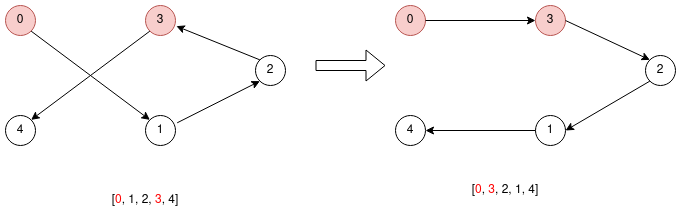
\includegraphics[width=\textwidth]{chapters/literature/img/2exdrawio.png}
      \caption{Przykład procedury 2-exchange}
      \label{fig:2exchange}
\end{figure}






